In this chapter, the requirements of a system that can solve the problem described in the problem definition in chapter \ref{problemdefinition} has been defined. The goal is to produce a requirement specification.

First the roles of the different kinds of users that will use the system has been defined. The system behavior has then been defined for the part handling falling accidents. Finally the requirements are defined, using a MoSCoW analysis.

\section{User Roles}\label{sec:user-roles}
The system is designed around multiple types of users, each of which has their own role with different responsibilities. For this purpose, four user types has been defined: Citizen, Contact, Citizen Admin and User Admin. The responsibility of each has been described in the following sections.

\subsection{Citizen}
The citizen role represents the elderly people at risk of having a falling accident. They are the group that has been researched and described in chapter \ref{preliminaries:problemanalysis}. Their ability in the system should be to activate alarms when they have had a falling accident.

\subsection{Contact}
The contact role defines the group of people that can help citizens, who have had a falling accident. They do not have to be associated with a citizen.

\subsection{Citizen Admin}
The Citizen Admin is responsible for creating and managing the citizens in the system. They can manage multiple citizens, and can update their information and assign contacts. It was chosen to separate this functionality from the citizen, to minimize confusion and errors that might come from this. It is possible for a physical user of role citizen, to be a citizen admin as well, if the user has the technical skills to manage this.

\subsection{User Admin}
The User Admin role is for people who manage the system itself. They have access to view and manage all users, devices and alarms. They interact with the system through a web interface, such that the administrative part of the system does not have to work directly in the database in order to view or change things.

\section{System behaviour}\label{sec:system-behaviour}
To better understand how the system developed throughout this report could be designed, this section contains descriptions of actual situations that the system could be used in. This includes descriptions of how each part of the system should respond to an event.

The system should be activated upon one of the following conditions, that triggers during or after the falling accident has happened:

\begin{itemize}
    \item A citizen activates the system manually
    \item A smartphone detects a falling accident
    \item A personal assistant detects a falling accident
\end{itemize}

When a smartphone detects a falling accident it should wait a duration for user response, either in the form of a button press or voice detection. This would allow for the user to interrupt the process, and avoid contacts being contacted when not needed. When a duration has passed and no user interaction has happened, the system notifies all contacts associated with the citizen.

A diagram showing this interaction can be found figure \ref{fig:SmartPhoneApp}. The figure shows the interaction between the citizen and contact, through the system. Dashed lines represent alternative paths. The timeout represents a system timeout, that activates the alarm, if no input is given by the user before it runs out. This syntax is used through out the rest of this chapter.

\begin{figure}[H]
    \centering
    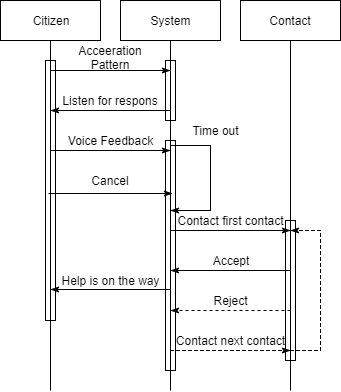
\includegraphics[width=0.5\textwidth]{Figures/Phone.png}
    \caption{Sequence diagram for smartphone app}
    \label{fig:SmartPhoneApp}
\end{figure}

When a personal assistant detects a falling accident, it should verify whether or not a falling accident has actually taken place. If a falling accident has happened, the system should notify the contacts associated to the citizen that has had the accident. The personal assistant should be context aware, such that it does not call for help during normal dialogue, and in general try to distinguish between false positives. This process can be seen on graph \ref{fig:PersonAssitent}. Sequences in quotes represent speech.

\begin{figure}[H]
    \centering
    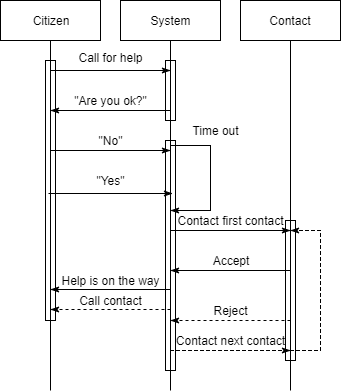
\includegraphics[width=0.5\textwidth]{Figures/PersonAssitent.png}
    \caption{Sequence diagram for personal assistant}
    \label{fig:PersonAssitent}
\end{figure}


The system will notify contacts, through their chosen device. When using the app they should have the option of responding whether they can help or not, and in the case that they can help, the system should notify the citizen that help is on its way.

Apart from the above behaviours, the system should behave as follows when configuring new users and devices. The new user must be configured through a web interface. When a user is added, it is necessary to include enough information such that it is possible to identify the user. Each citizen has a list of contacts that the system will contact in case of a fall accident.

A new fall detection device can be configured for the user. It is however not required that a user has a device. The app should however add itself as a device when the user login and remove itself again when the user logout.

Devices can be either a smartphone, a voice-assistant configured for fall detection, or other IoT enabled devices. These devices are coupled to a specific user upon configuration.

\subsection{Quantitative requirements}\label{sec:q-requirements}
To be able to validate the system, it is necessary to define some quantitative values that can be measured and compared to validate whether the system lives up to the requirements. Two values that can be defined are the amount of false positives allowed and the amount of false negatives allowed.

A false negative is when the system fails to register that a citizen has fallen.
 
Two types of false positives can be considered. The first is when the system registers a fall accident, but the citizen has not fallen and cancels before an alarm is sent. The second is when the citizen is not aware that the system has registered a falling accident and therefore does not cancel it. An example could be that the devices detects a fall accident, but the device is in the citizens bag. The accident is not canceled and the citizens contacts are faulty notified.

False negatives can have severe consequences for the user and must be avoided. To perceive the system as a success it cannot have any false negatives, as long as the system is used as designed. To be able to adhere to this, the system allows for more falls positives.

As described in \ref{sec:lifeLine}, the solution \textit{Lifeline} \cite{AAlert} claims that they have an accuracy of 95\%, meaning that 5\% of their alarms are false positive. Considering the non-tolerance for false negatives, this percentage is acceptable for the system, when measuring the second type of false positives. If the system is used as intended, there should not be any false positives of the first type, since the citizen can cancel the alarm before it is activated.

\section{MoSCoW analysis}\label{sec:moscow}
From the system behaviour explored, throughout this chapter, and the quantitative requirements defined, a requirement specification has been formulated. The requirements define the functionality required for the system to be considered a success. To prioritize the requirements a MoSCoW analysis has been made.

MoSCoW is a method for prioritizing requirements, where the requirements are organized into four categories: \textit{must have}, \textit{should have}, \textit{could have} and \textit{won't have}.
\textit{Must have} covers the requirements that are critical for the system to be considered a success. \textit{Should have} covers the requirements that are still important, but not critical for the system to be a success. \textit{Could have} covers the requirements that can improve the user experience, but are only added if time allows. \textit{Won't have} covers the requirements that are dropped or moved to a later release, but they may still be important for the system overall.

\textbf{Must have}
\begin{itemize}
    \item[1] Functionality to add and administrate citizens without need for a system administrator.
    \item[2] Detect when a citizen has had a fall accident, through input from the user on a device, such as a smartphone or wearable.
    \item[3] Send an alarm to all of the citizen's contacts.
\end{itemize}

\textbf{Should have}
\begin{itemize}
    \item[4] Detect when a citizen has had a fall accident, through conversation with a personal assistant.
    \item[5] Facilitate communication between a citizen and contact person during a fall accident.
\end{itemize}

\textbf{Could have}
\begin{itemize}
    \item[6] Be able to integrate IoT devices.
        \begin{itemize}
            \item[6.1] Associate device with a citizen to send alarms using device.
            \item[6.2] Associate device with a contact person to receive alarms using device.
        \end{itemize}
\end{itemize}

\textbf{Won't have}
\begin{itemize}
    \item[7] Automatically detect when a citizen has had a fall accident, using a smartphone.
    \item[8] Have a high accuracy when detecting a fall accident, as defined in section \ref{sec:q-requirements}.
\end{itemize}


Requirements 4 and 5 has been defined as \textit{should have} since they are not considered core requirements for the system to be successful.

Requirement 6 has been defined as \textit{Could have}, since it is a \textit{nice to have} feature, but is outside the scope of this project.

Requirement 7 has been defined as \textit{Won't have}, since it is not the focus for this project. Requirement 8 is dependent of requirement 7, and therefore is also defined as \textit{Won't have}.